\documentclass[border=0.15cm]{standalone}
\usepackage{tikz}
%\usetikzlibrary{positioning}
\usetikzlibrary{arrows,shapes,positioning}
\usetikzlibrary{calc,decorations.markings}
%\usetikzlibrary{calc,decorations.markings}
\usetikzlibrary{shapes.geometric, arrows}
\tikzstyle{startstop} = [rectangle, rounded corners, minimum width=3cm, minimum height=1cm,text centered, draw=black, fill=red!30]
\tikzstyle{io} = [trapezium, trapezium left angle=70, trapezium right angle=110, minimum width=0.5cm,text width = 1.5cm, minimum height=1cm, text centered, draw=black, fill=blue!30]
\tikzstyle{process} = [rectangle, minimum width=2cm, minimum height=1cm, text width = 2cm, text centered, draw=black, fill=orange!30]

\tikzstyle{process2} = [rectangle, minimum width=3cm, minimum height=1cm, text centered, draw=black, fill=green!30]

\tikzstyle{process3} = [rectangle, minimum width=3cm, minimum height=1cm, text centered, draw=black, fill=blue!30]

\tikzstyle{decision} = [diamond, minimum width=3cm, minimum height=1cm, text centered, draw=black, fill=green!30]
\tikzstyle{arrow} = [thick,->,>=stealth]

\tikzset{
 % block/.style={rectangle, draw, fill=blue!10, rounded corners, text centered,     text width = 7em, minimum height = 2em},
  line/.style={draw, -latex'}
  }

\definecolor{burntorange}{cmyk}{0,0.52,1,0}
\tikzstyle{legend_general}=[rectangle, rounded corners, thick,
                           burntorange, fill= green!5, draw, text=violet,
                           minimum width=2.5cm, minimum height=0.8cm]
\begin{document}
%\begin{minipage}[h]{0.49\linewidth}
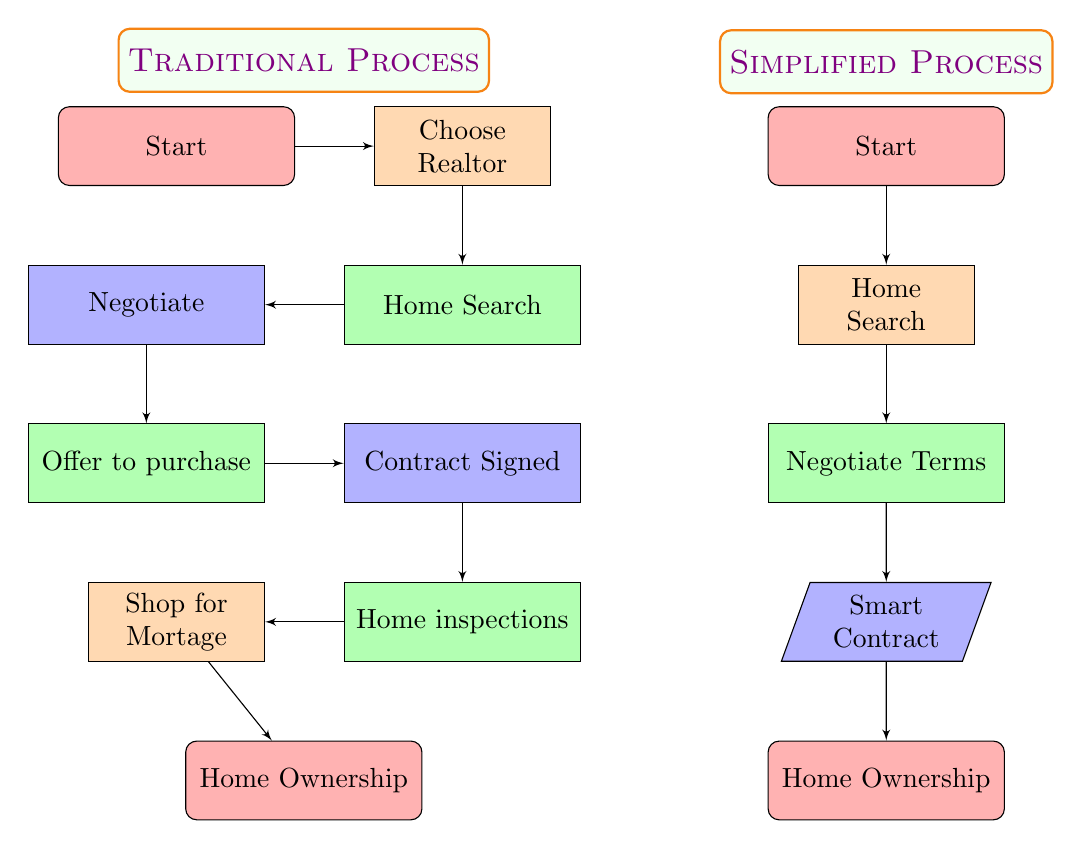
\begin{tikzpicture}

\node (start) [startstop] {Start};

\node (in1) [process, right = 1cm of start] {Choose Realtor};

\node (in2) [process2, below =1cm of in1] {Home Search };
\node (in3) [process3, left = 1cm of in2] {Negotiate};

\node (in4) [process2, below = 1cm of in3] {Offer to purchase};

\node (in5) [process3, right = 1cm of in4] {Contract Signed};

\node (in6) [process2, below = 1cm of in5] {Home inspections};

\node (in7) [process, left = 1cm of in6] {Shop for Mortage};

\node (in8) [startstop, below left=1cm and -1cm of in6] {Home Ownership};
\foreach \x/\y in {start/in1,
                   in1/in2,
                   in2/in3,
                   in3/in4,
                   in4/in5,
                   in5/in6,
                   in6/in7,
                   in7/in8}
   \draw [line] (\x) -- (\y);

\node (start2) [startstop, right =6cm of start] {Start};

\node (inSM1) [process, below =1cm of start2] {Home Search};

\node (inSM2) [process2, below =1cm of  inSM1] {Negotiate Terms};

\node (inSM3) [io, below =1cm of  inSM2] {Smart Contract};

\node (inSM4) [startstop, below =1cm of  inSM3] {Home Ownership};

\foreach \x/\y in {start2/inSM1,
                   inSM1/inSM2,
                   inSM2/inSM3,
                   inSM3/inSM4}
   \draw [line] (\x) -- (\y);
   
% Legend pictures 
\node[legend_general,above =8.225cm of in8] {{\large \textsc{Traditional Process}}};
\node[legend_general,above = 0.15 cm of start2] {{\large \textsc{Simplified Process}}};
\end{tikzpicture}

%\end{minipage}
%\begin{minipage}[h]{0.49\linewidth}
%\begin{tikzpicture}[node distance=2cm]



%\end{tikzpicture}

%\end{minipage}
\end{document}